CAP teorien blev først udgivet i 1999 som en databaseteori, hvoraf man kan udlede, at ved valg af en database til et system, kan man vælge to ud af de tre garantier som set på figur \ref{fig::CAP}. Udgivelsen af teorien har medført kritik af dets hypotese om, at et databasesystem kun kan opfylde to af de tre garantier. Kritikken er relevant da de fleste databaser i nyere tid går efter at opnå alle tre garantier. 
Ser man på visualiseringen af CAP theorem på figur 1 ses tre punkter, disse punkter står således for nogle garantier, som systemet vil kunne levere. Consistency står for at hvert element man anmoder om giver det seneste opdateret resultat, eller en fejl. Availability står for at hver forespørgsel får et svar, uden at garantere at det er det seneste opdateret resultat. Til sidst står partition tolerence for at systemet kan fortsætte med at fungere på trods af at et vilkårligt antal af beskeder bliver tabt eller forsinket mellem partitionerne, f.eks. ved netværksfejl. Den almindelige MySQL database vil ligge op ad availability og consistency, mens de fleste, og specielt cloud baserede NoSQL databaser vil ligge sig op ad availability og partition tolerance. Det er dog kun under en netværksfejl man vil være nødt til at gå på kompromi med enten availability eller consistency. Den bygger dog stadig et godt fundament til argumentation for hvad for en database man skal vælge, og kigge på deres fordele og ulemper.
\begin{figure}
    \centering
    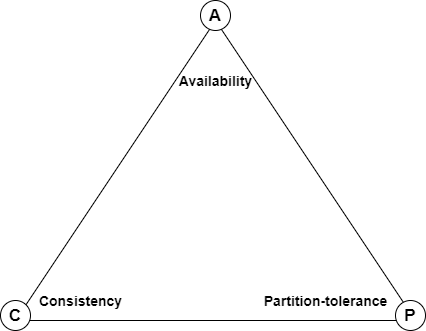
\includegraphics[scale=0.8]{CAP.png}
    \caption{CAP Theorem illustreret.}
    \label{fig::CAP}
\end{figure}